%!TeX root=../tese.tex
%("dica" para o editor de texto: este arquivo é parte de um documento maior)
% para saber mais: https://tex.stackexchange.com/q/78101/183146

\chapter{Conclusion}
\label{cap:conclusion}

In this work, we studied recommender system bias. As detailed in
Chapter~\ref{cap:introduction}, these algorithms are pervasive in modern live
and have significant impact on our information diet; however, a growing body of
evidence indicates that these systems, specially when deployed in large social
networks, can display significant biases in their recommendations. Researchers
and activists alike worry that these bises might create echo chambers and
radicalization pipelines by amplifying extremist content. In broad terms, our
goal was to study one way through which these algorithms might be boosting
fringe viewpoints and radicalizing users: degenerate feedback loops.

Degeneracy in recommender systems has been explored before by
\citet{nguyen_exploring_2014} and \citet{jiang_degenerate_2019}. They concluded
that these algorithms show a tendency to reduce the diversity of recommended
content over time because of the feedback loop that occurs when the system must
learn from the its own outputs. Our main research objective was to further
characterize and model this behavior using both qualitative and quantitative
methods.

In Chapter~\ref{cap:review}, we reviewed the scientific literature that deals
with this topic and presented a few different viewpoints on the matter. Works by
\citet{hosseinmardi_evaluating_2020}, \citet{huszar_algorithmic_2021}, and
others suggest that social networks tend to amplify far-right views, while
\citet{munger_right-wing_2020} and \citet{ledwich_algorithmic_2019} posit that
this is not the case. \citet{ribeiro_auditing_2020} found evidence that, in
general, YouTube users tend to migrate from "lighter" content towards more
extreme videos, and \citet{stoica_algorithmic_2018} coined the term
``algorithmic glass ceiling'' to describe recommender system's propensity to
reinforce homophilic behavior.

We also drew attention to non-scientific endeavors that attempt to better
understand filter bubbles, echo chambers, and their impacts on the public. While
this issue is being debated in academia, journalists and whistleblowers like
\citet{ribeiro_como_2021} or \citet{wong_how_2021} hold social media companies
accountable by gathering anecdotal evidence and personal accounts about
algorithmic bias.

Our main contributions come in Chapters~\ref{cap:static} and \ref{cap:dynamic},
where we describe and conduct multiple experiments on recommender algorithms.

\section{Static Analysis}
\label{sec:static}

Chapter~\ref{cap:static} started with a question: can recommender systems send
users in radicalization spirals? Given the many limitations of social media
analysis, we argue that the best way to answer this question is to explore the
simplest and most bare-bones algorithm possible. Our hypothesis is that, if such
a simple algorithm displays a feedback loop dynamic, then there might be some
intrinsic property of this type of system that pushes recommendations towards
degeneracy.

We designed multiple experiments with the goal of analyzing the recommendation
profile of our algorithm of choice: a simple, content-based recommender that
used cosine similarity as its internal metric. Recommendation profile is a
concept we developed as a shorthand for an algorithm's characteristic tendency
to recommend more frequently a smaller (or larger) subset of the original data.

Our expectation was that a systems's recommendation profile would be
approximately the same as the original dataset's item popularity distribution;
users that enjoyed less popular movies would be recommended other unpopular
items and users that enjoyed the more popular movies would likewise be
recommended other prominent items. This, however, was not the case.

In the original MovieLens \citep{harper_movielens_2015} dataset, the popularity
distribution was sub-exponential, meaning that there was not a sharp decrease in
the number of reviews from the most popular movies to the least popular ones.
This was in stark contrast to our vanilla model's exponential recommendation
profile. Figure ~\ref{fig:fig05_profile_comparison} displays the two profiles
side-by-side for ease of reference.

\begin{figure}
  \centering
  \begin{subfigure}{0.45\textwidth}
    \centering
    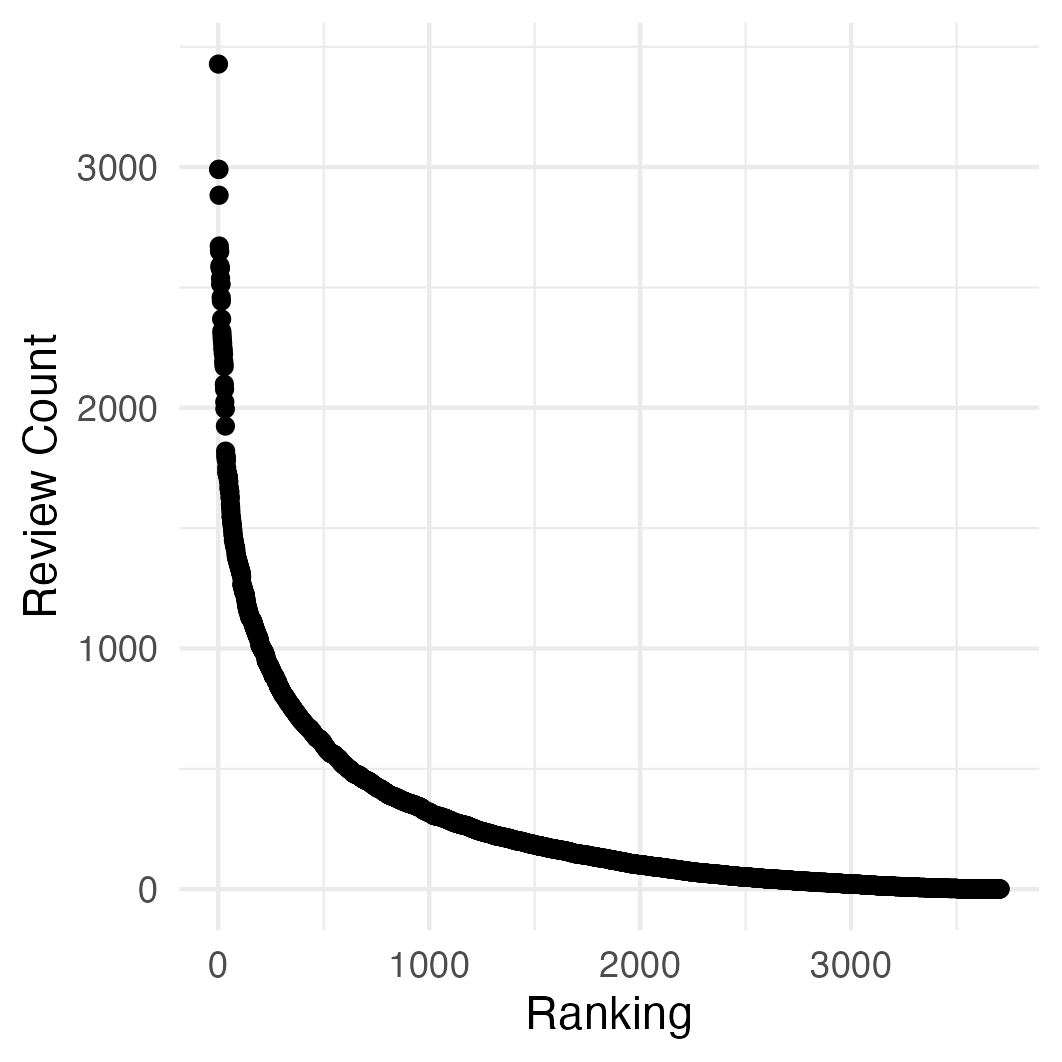
\includegraphics[width=\textwidth]{03_review_profile}
    \caption{Popularity distribution.\label{fig:fig05_review_profile}}
  \end{subfigure}
  \begin{subfigure}{0.45\textwidth}
    \centering
    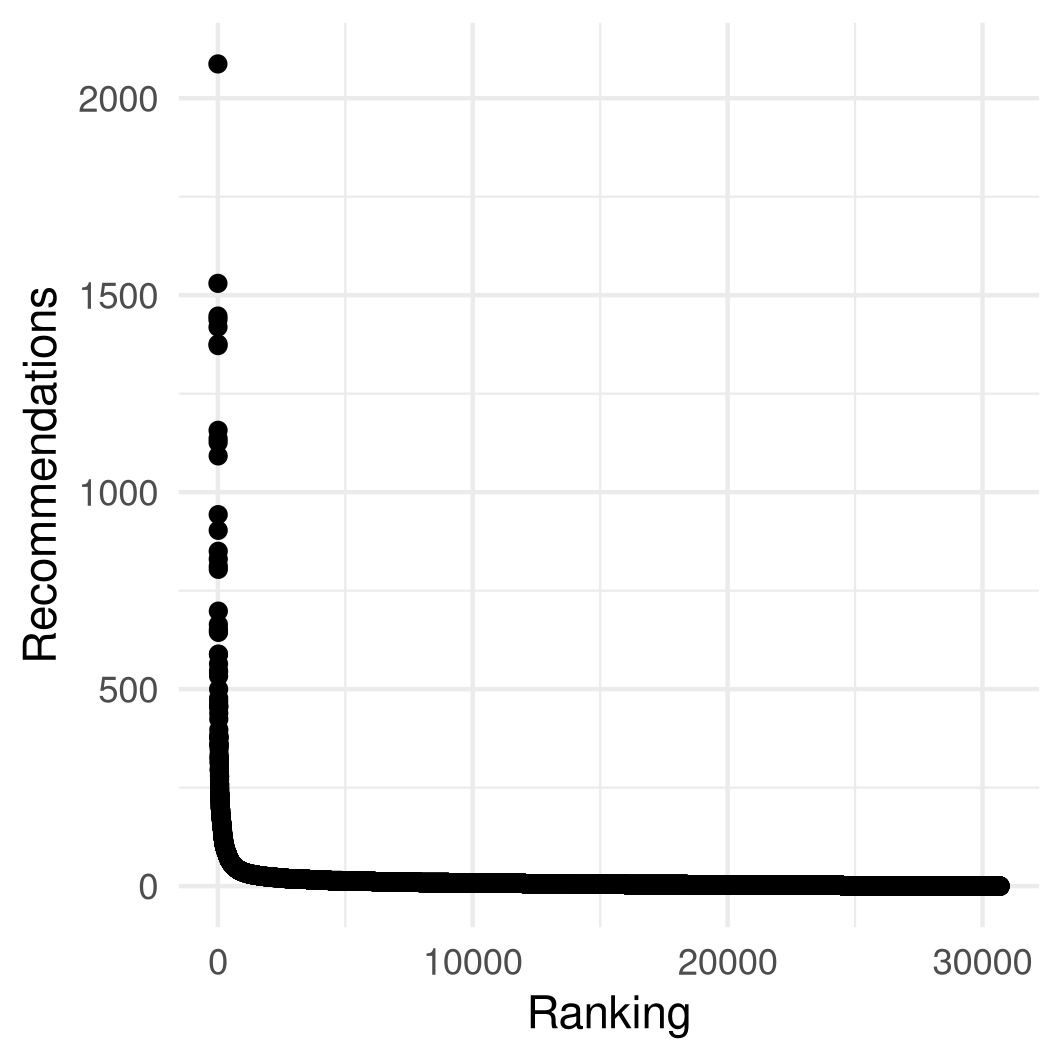
\includegraphics[width=\textwidth]{2a_vanilla}
    \caption{Recommendation profile.\label{fig:fig05_vanilla_profile}}
  \end{subfigure}
  \caption{Comparison between the original dataset's review profile (a) and the
  vanilla algorithm's recommendation
  profile.\label{fig:fig05_profile_comparison}}
\end{figure}

We experimented on many variations to the vanilla model and of the original
dataset, but all of them displayed exponential or super-exponential
recommendation profiles. This led us to posit that, indeed, recommender systems
might be prone to artificially amplifying some contents independently of the
original data. However, this static analysis was only part of the story and, in
order to confirm this hypothesis, we needed to take user dynamics into account.

\section{Dynamic Analysis}
\label{sec:dynamic}

We followed up the static experiments with a dynamic analysis. The main
question that motivated Chapter~\ref{cap:dynamic} was whether the amplification
pipeline detected in Chapter~\ref{cap:static} would be even further emphasized
by the interaction between user and recommendation system.

Even though we used a bare-bones algorithm again, this time we went with
Google's own machine learning library: TensorFlow Recommenders
\citep{noauthor_tensorflow_nodate}. Our goal was to capture the dynamics that
arise when a machine learning system has to learn from its own data, i.e., the
engagement of a user with items recommended by the algorithm itself. Since we
needed to generalize our conclusions to the environment of a social network, the
library Google uses to build its recommendation engines was the ideal choice.

Using the same MovieLens \citep{harper_movielens_2015} dataset, we created a
loop where the system would recommend 10 movies to a simulated user, this user
would then chose one movie at random to "watch", and this interaction would be
fed back into the model as a new input. This process was repeated 5 times for
each user in the original dataset.

Just as with the static experiments, the recommendation profile of our algorithm
got steeper and steeper over time, resulting in a similar super-exponential
decay; a diminishing set of movies was being recommended to a growing number of
users (as can be seen in Figure~\ref{fig:fig05_amplification}). Interestingly,
the movies that grew in popularity with time were not the most popular ones in
the original dataset.

In order to better understand the progression of the recommendation profile, we
tried to model this behavior using well-understood statistical distributions. If
we were able to accurately reproduce the results we obtained from the machine
learning algorithm with a white-box model, we would gain a deeper insight into
the internal mechanisms that caused the amplification pipeline we were
detecting.

\begin{figure}
  \centering
  \begin{subfigure}{0.45\textwidth}
    \centering
    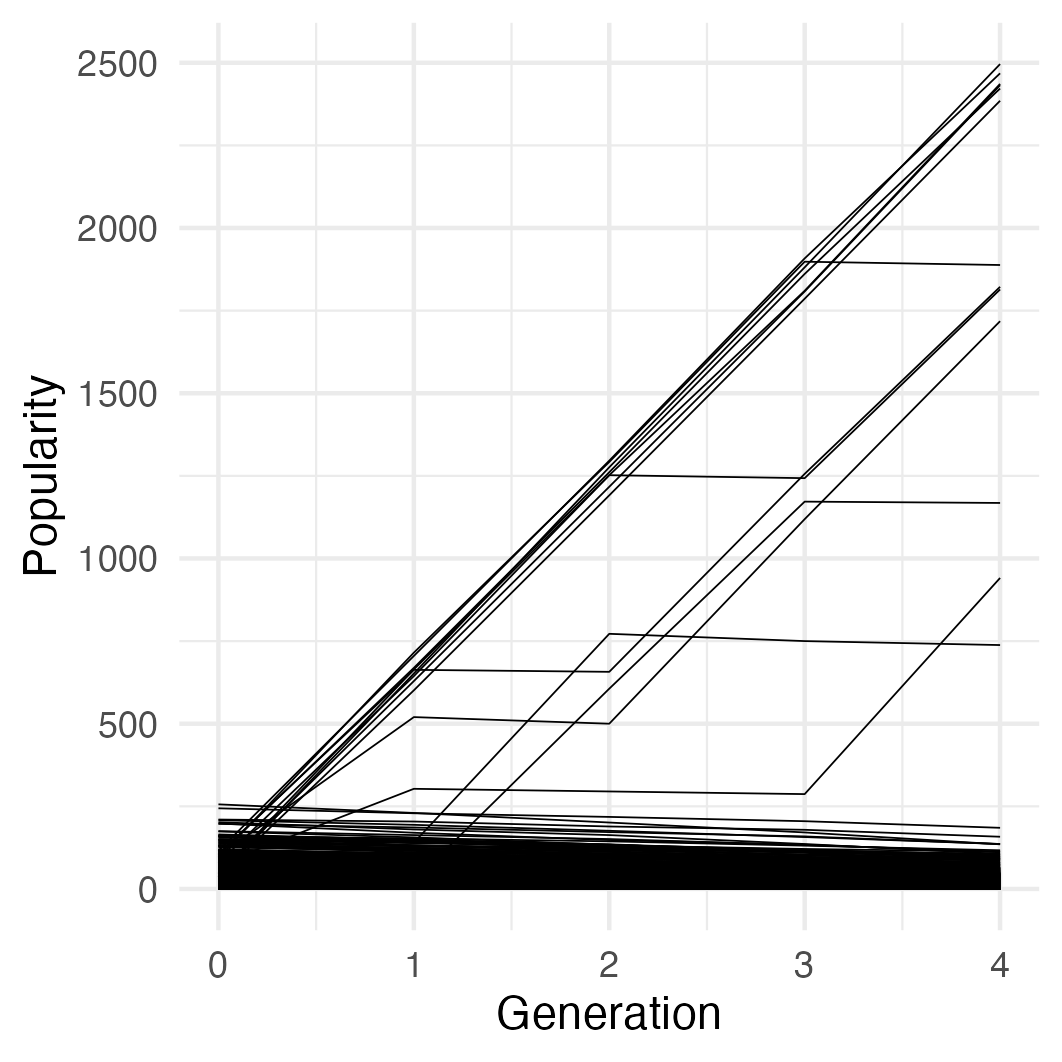
\includegraphics[width=\textwidth]{04_popularity_time}
    \caption{Movie popularity over time.\label{fig:fig05_popularity_time}}
  \end{subfigure}
  \begin{subfigure}{0.45\textwidth}
    \centering
    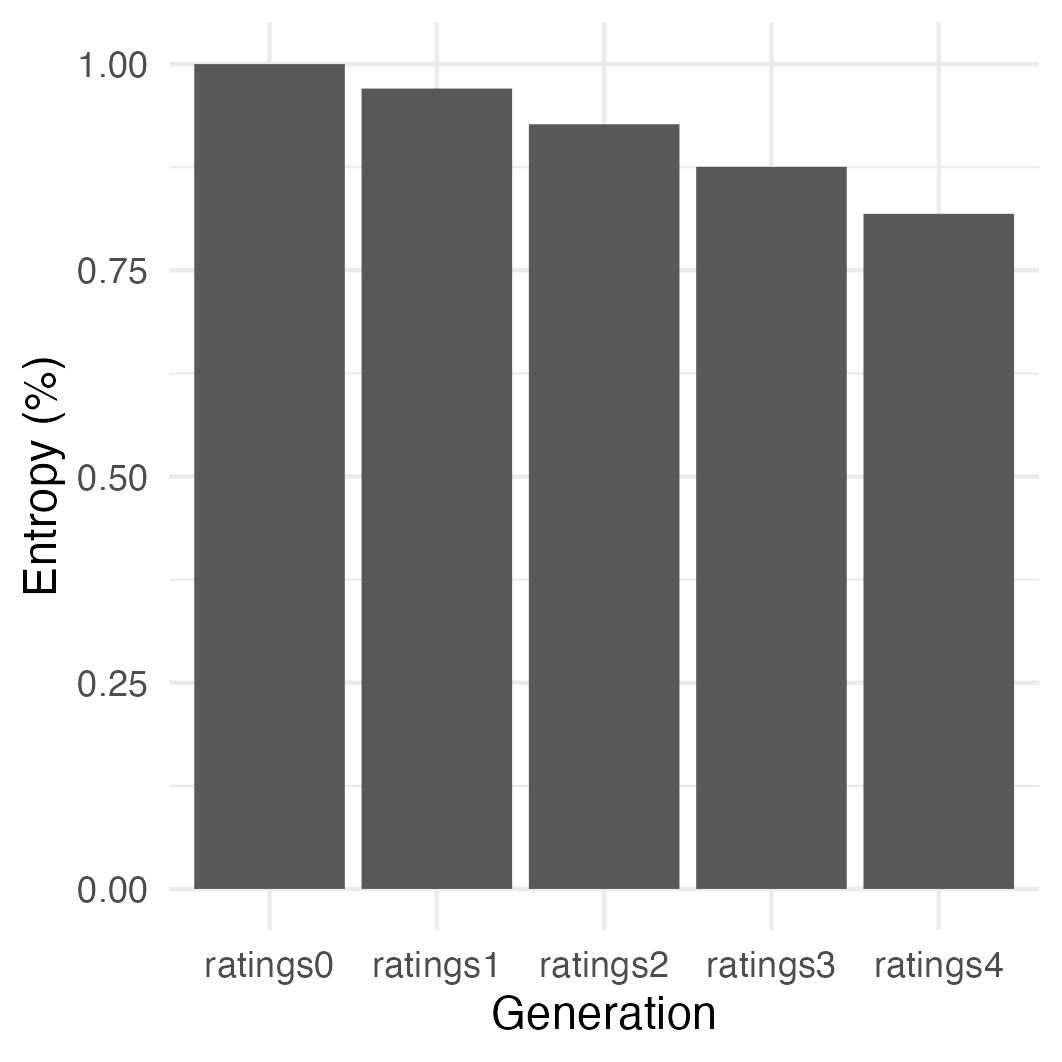
\includegraphics[width=\textwidth]{04_entropy}
    \caption{Recommendation entropy over time.\label{fig:fig05_entropy}}
  \end{subfigure}
  \caption{Amplification pipeline detected on the dynamic
  experiment.\label{fig:fig05_amplification}}
\end{figure}

We attempted to model the pipeline with Poisson and negative binomial
regressions, but had no success in both cases. We also tried adding
mixed-effects to these models and were better able to capture the variance of
the phenomenon, but a simulated envelope analysis revealed that our attempts
were still falling short.

As with the numbers obtained by \citet{} in a different scenario, the % Degenerate feedback loops in recommender systems
recommendation profiles of our model were tending quickly towards a degenerate
distribution. We believe that this is yet another piece of evidence that
suggests that recommender systems, if left unchecked, tent towards a confinement
dynamic where users' feeds devolve into filter bubbles and where the points of
view of highly-engaged minorities are amplified by a system that has to learn
from itself.

\section{Final Remarks}
\label{sec:remarks}

We began this work with the goal of developing a better understanding of the
mechanisms through which recommendation algorithms could be radicalizing users,
creating echo chambers and boosting fringe viewpoints. We believe we have found
enough evidence to support the hypothesis that recommender systems are able to
create amplification pipelines from degenerate feedback loops.

However, our findings are but one step in the direction of a solid theory.
Further research is still needed in order to find an unambiguous causal between
these processes and, more importantly, how to fix this behavior. A possible next
step would involve applying the methods discussed in this work to more complex
recommendation systems and to larger real-world datasets.
